% Cover
\imprimircapa

% False cover sheet
%\imprimirfalsafolhaderosto

% Cover sheet
\imprimirfolhaderosto

% Card Catalog
\begin{fichacatalografica}
	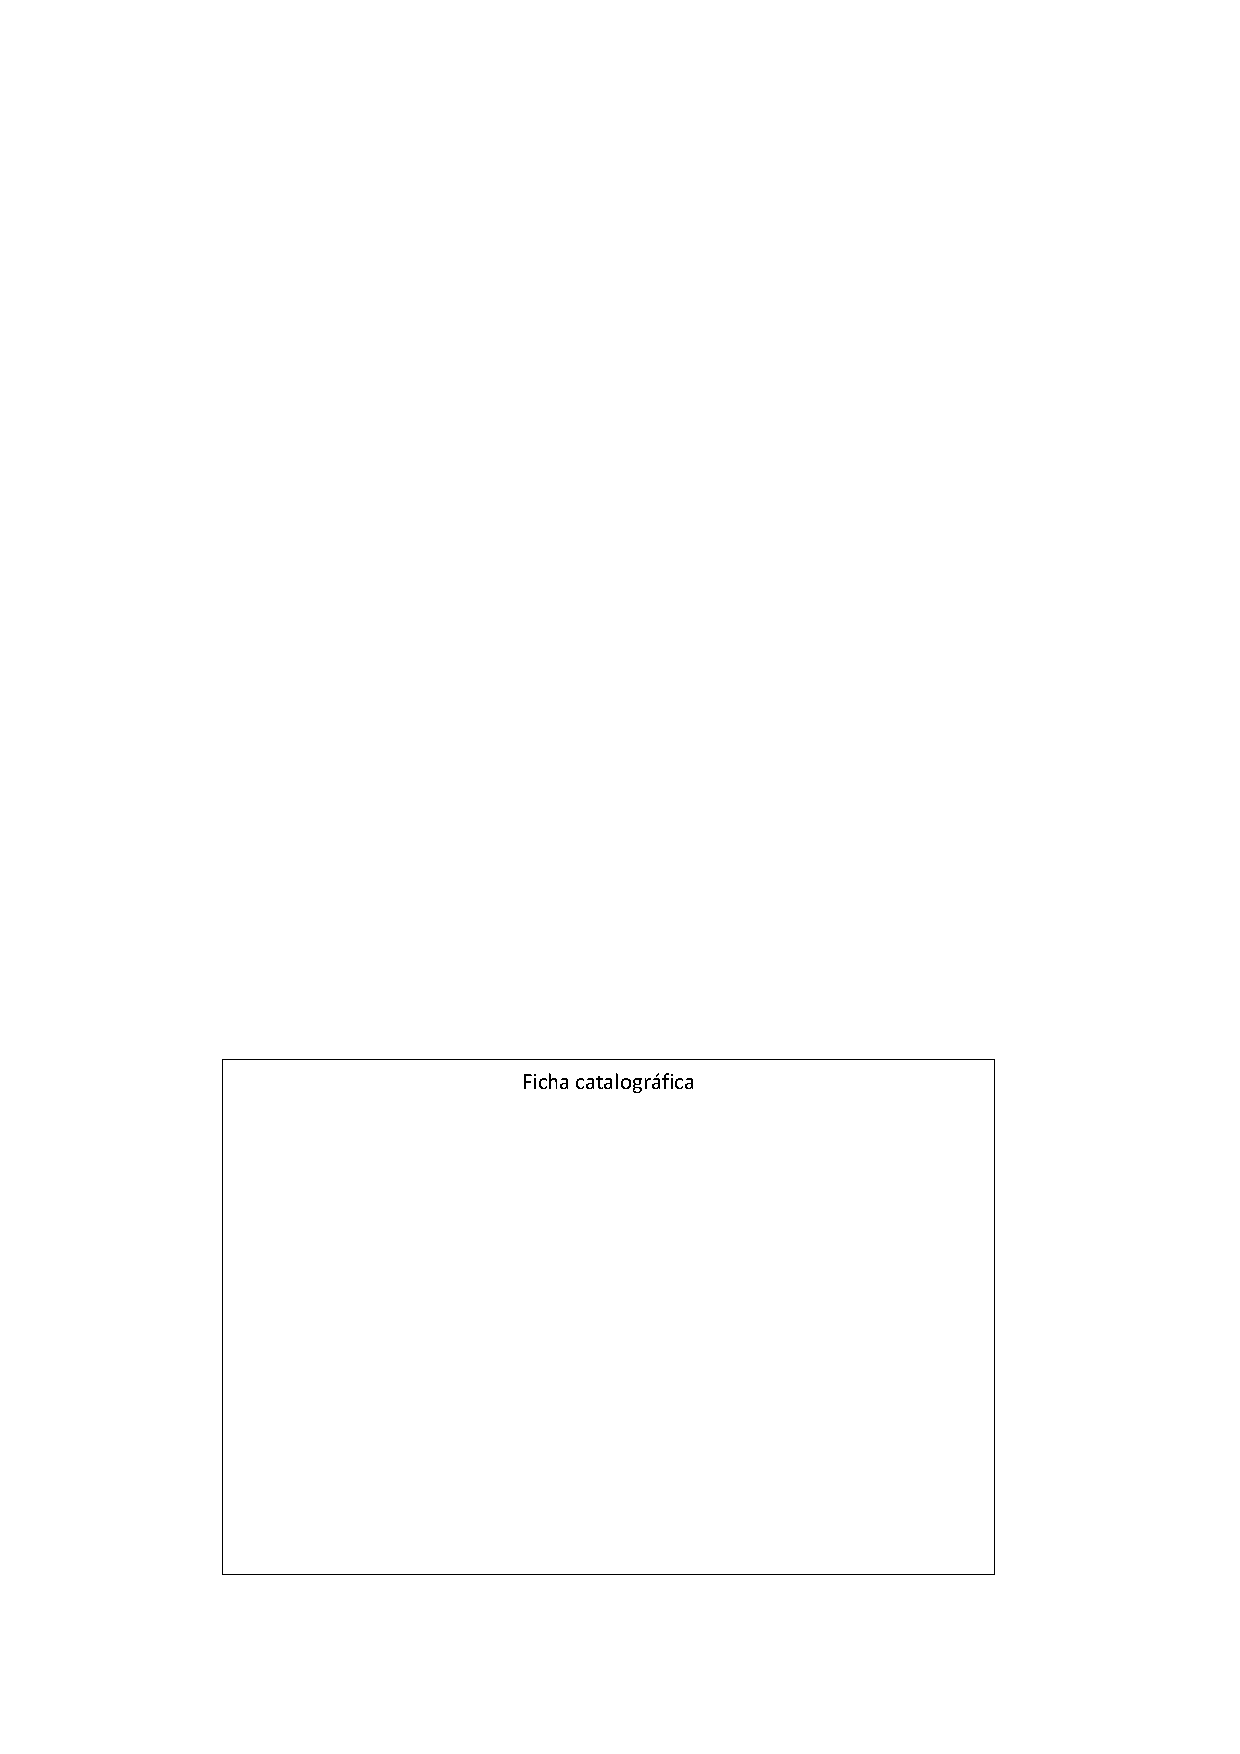
\includepdf{card-catalog.pdf}
\end{fichacatalografica}

% Approval sheet
%\begin{folhadeaprovacao}
%	
%	\begin{center}
%		{\ABNTEXchapterfont\large\imprimirautor}
%		
%		\vspace*{\fill}\vspace*{\fill}
%		\begin{center}
%			\ABNTEXchapterfont\bfseries\Large\imprimirtitulo
%		\end{center}
%		\vspace*{\fill}
%		
%		\hspace{.45\textwidth}
%		\begin{minipage}{.5\textwidth}
%			\imprimirpreambulo
%		\end{minipage}%
%		\vspace*{\fill}
%	\end{center}
%	
%	%Trabalho aprovado. \imprimirlocal, 31 de dezembro de 2020:
%	
%	\assinatura{\textbf{\imprimirorientador} \\ Orientador} 
%	\assinatura{\textbf{\imprimircoorientador} \\ Coorientador} 
%	\assinatura{\textbf{A} \\ Convidado 1}
%	\assinatura{\textbf{B} \\ Convidado 2}
%	
%	\begin{center}
%		\vspace*{0.5cm}
%		{\large\imprimirlocal}
%		\par
%		{\large\imprimirdata}
%		\vspace*{1cm}
%	\end{center}
%	
%\end{folhadeaprovacao}

% Abstract - Portuguese
\setlength{\absparsep}{18pt} % Spacing
\begin{resumo}
	Indústria 4.0 (I4.0) se refere às recentes modificações em relação às tecnologias de manufatura. Neste contexto, redes inteligentes de máquinas passam a proporcionar um alto nível de automação e intercâmbio de informações entre equipamentos, produtos e demais atores em um ambiente de manufatura. Visto a relevância do compartilhamento de informações para a implementação de soluções no contexto da I4.0 conforme apontado pela bibliografia, este trabalho aborda este tema, mais especificamente o compartilhamento da memória digital do produto (MDP) ao longo da cadeia de suprimentos (CS). Para isso, é elaborada de uma arquitetura baseada no Modelo de Arquitetura de Referência para a Indústria 4.0 (RAMI4.0). Nesta arquitetura, a MDP é compartilhada por meio de \textit{Web Services} e é composta por três componentes básicos: o servidor de informações (o produto), o cliente consumidor de informações (cada elo da CS) e o repositório, que contém as descrições dos serviços ofertados. Além disso, este trabalho aborda a modelagem de dados dos submodelos de um Componente 4.0 (C4.0) e considerações sobre o impacto em geração de valor que este amplo compartilhamento durante o ciclo do produto traz sobre o negócio. Por fim, o resultado deste trabalho é a modelagem desta arquitetura pela qual permite-se padronizar a forma de interação entre os elos de uma CS, garantindo assim a interoperabilidade entre eles.

	\vspace{\onelineskip}

	\noindent
	\textbf{Palavras-chave}: Indústria 4.0. RAMI4.0. Memória digital do produto. Arquitetura orientada a serviços. Cadeia de suprimentos.
\end{resumo}

% Abstract - English
\begin{resumo}[Abstract]
	\begin{otherlanguage*}{english}
		Industry 4.0 (I4.0) refers to the recent changes in manufacturing technologies. In this context, intelligent machine networks provide a high level of automation and information exchange between equipments, products and other actors in a manufacturing environment. Given the relevance of information sharing for the implementation of solutions in the context of I4.0 as pointed out by the bibliography, this work addresses this topic, more specifically the sharing of the Digital Product Memory (DPM) along the supply chain (SC). For this, an architecture based on the Reference Architectural Model Industrie 4.0 (RAMI4.0) is developed. In this architecture, the DPM is shared through \textit{Web Services} and is composed of three basic components: the information server (the product), the information consumer (each CS link) and the repository, which contains descriptions of the offered services. In addition, this work addresses the data modeling of the submodels of a Component 4.0 (C4.0) and considerations about the impact on value generation that this broad sharing during the product lifecycle brings to the business. Finally, the result of this work is the modeling of this architecture through which it is possible to standardize the way of interaction between the members of a SC, thus ensuring interoperability between them.
		\vspace{\onelineskip}

		\noindent
		\textbf{Keywords}: Industry 4.0. RAMI4.0. Digital product memory. Service-oriented architecture. Supply chain.
	\end{otherlanguage*}
\end{resumo}

% List of illustrations
\pdfbookmark[0]{\listfigurename}{lof}
\listoffigures*
\cleardoublepage

% List of tables
\pdfbookmark[0]{\listtablename}{lot}
\listoftables*
\cleardoublepage

% List of abbreviations and acronyms
\begin{siglas}
	\item[AAS] \textit{Asset Administration Shell} (Casca Administrativa do Ativo)
	\item[API] \textit{Application Programming Interface} (Interface de Programação de Aplicação)
	\item[BD] Banco de Dados
	\item[BI] \textit{Business Intelligence} (Inteligência Empresarial)
	\item[BOM] \textit{Bill of Materials} (Lista de Materiais)
	\item[C4.0] Componente 4.0
	\item[CRUD] \textit{Create, Read, Update, Delete} (Criação, Leitura, Atualização, Exclusão)
	\item[CS] Cadeia de Suprimentos
	\item[CV] Cadeia de Valor
	\item[CVP] Ciclo de Vida do Produto
	\item[GCVP] Gestão do Ciclo de Vida do Produto
	\item[GI] Gestão da Informação
	\item[I4.0] Indústria 4.0
	\item[IIoT] \textit{Industrial Internet of Things} (Internet das Coisas Industrial)
	\item[IoT] \textit{Internet of Things} (Internet das Coisas)
	\item[JSON] \textit{JavaScript Object Notation} (Notação de Objeto do JavaScript)
	\item[LGPD] Lei Geral de Proteção de Dados
	\item[MDP] Memória Digital do Produto
	\item[OEE] \textit{Overall Equipment Effectiveness} (Eficiência Global do Equipamento)
	\item[OSI] \textit{Open System Interconnection} (Interconexão Aberta de Sistemas)
	\item[PFS] \textit{Production Flow Schema} (Esquema de Fluxo de Produção)
	\item[QoS] \textit{Quality of Service} (Qualidade de Serviço)
	\item[RAMI4.0] \textit{Reference Architectural Model Industrie 4.0} (Modelo de Arquitetura de Referência para a Indústria 4.0)
	\item[REST] \textit{Representational State Transfer} (Transferência Representacional de Estado)
	\item[RFID] (\textit{Radio-Frequency IDentification}) (Identificação por Radiofrequência)
	\item[SOA] \textit{Service Oriented Architecture} (Arquitetura Orientada a Serviços)
	\item[SOAP] \textit{Simple Object Access Protocol} (Protocolo para Simples Acesso de Objetos)
	\item[SED] Sistemas a eventos discretos
	\item[TIC] Tecnologia da Informação e Comunicação
	\item[UUID] \textit{Universal Unique IDentifier} (Identificador Único Universal)
	\item[WS] \textit{Web Service} (Serviço Web)
	\item[WSD] \textit{Web Services Description} (Descrição do Serviço Web)
	\item[WSDL] \textit{Web Services Description Language} (Linguagem de Descrição de Serviços Web)
	\item[XML] \textit{Extensible Markup Language} (Linguagem Extensível de Marcação)
\end{siglas}

% Summary
\pdfbookmark[0]{\contentsname}{toc}
\tableofcontents*
\cleardoublepage
